% !TEX root = ../HonoursThesis.tex

\renewcommand{\chapterlabel}{Chapter}
\chapter{Echo state network with ordinal partition based readout switching}
\label{chap:ORSESN}


The first approach uses a piecewise readout function to incorporate ordinal partition information into the structure of an ESN. In this architecture there is a different readout vector for each observed ordinal partition and at each time step, a readout vector is chosen depending on the partition of the input data. We will refer to this architecture as the Ordinal partition based Readout Switching ESN (ORSESN).

% \begin{figure}
%     \centering
%     \begin{tikzpicture}[scale=1.2]
%         \node[fill=col1,circle,inner sep=4pt,label=left:$\mathbf{x}(t)$] (input) at (0,0) {};
%         \node[fill=black,circle,inner sep=2pt,label=right:$\mathbf{y}(t)$] (output) at (10,0) {};
        
        
%         \coordinate (res_anchor) at (2,3);
%         \node[fill=black,circle,inner sep=2pt] (res1) at ({5-0.5},{0.8}) {};
%         \node[fill=black,circle,inner sep=2pt] (res2) at ({5},{-1}) {};
%         \node[fill=black,circle,inner sep=2pt] (res3) at ({5},{0.15}) {};
%         \node[fill=black,circle,inner sep=2pt] (res4) at ({5+1},{-0.1}) {};
%         \node[fill=black,circle,inner sep=2pt] (res5) at ({5-0.75},{-0.5}) {};
%         \node[fill=black,circle,inner sep=2pt] (res6) at ({5-1.25},{0.4}) {};
%         \node[fill=black,circle,inner sep=2pt] (res7) at ({5+0.65},{0.75}) {};
%         \node[fill=black,circle,inner sep=2pt] (res8) at ({5+1},{-0.9}) {};
%         \node[fill=black,circle,inner sep=2pt] (res9) at ({5-1.25},{-1}) {};
%         \node[fill=black,circle,inner sep=2pt] (res10) at ({5-1.75},{-0.25}) {};

%         \foreach \i in {1,...,10}
%             \draw[gray,line width=0.1] (input) -- (res\i);
        
%         \foreach \i in {1,...,5}
%             \foreach \j in {1,...,5} {
%                 \ifnum\i<\j
%                     \draw (res\i) -- (res\j);
%                 \fi
%             }
        
%         \draw (res6) -- (res5);
%         \draw (res6) -- (res1);
%         \draw (res6) -- (res10);
%         \draw (res10) -- (res5);
%         \draw (res9) -- (res10);
%         \draw (res9) -- (res2);
%         \draw (res7) -- (res1);
%         \draw (res7) -- (res3);
%         \draw (res7) -- (res4);
%         \draw (res8) -- (res4);
%         \draw (res8) -- (res2);
        
%         \foreach \i in {1,...,10}
%             \draw[gray,line width=0.1] (res\i) -- (output);
        
%         \begin{scope}[on background layer]
%         \draw[draw=black,fill=pale_yellow,rounded corners=8pt]  ($(res1)+(-0.1,0.3)$) -- ($(res7)+(+0.2,+0.2)$) -- ($(res4)+(0.4,0)$) -- ($(res8)+(0.2,-0.2)$) -- ($(res2)+(0,-0.2)$) -- ($(res9)+(-0.2,-0.2)$) -- ($(res10)+(-0.3,0)$) -- ($(res6)+(-0.3,0)$) -- cycle;
%         \end{scope}
%         \node at (5.2, 1.4) {$\mathbf{W}_{\text{rec}}$};
%         \node at (5, -1.6) {$\mathbf{s}(t)$};
        
%         \draw[fill=white,opacity=0.8] (1.2,-0.75) rectangle (2.0,0.75) node[midway] {$\mathbf{W}_{\text{in}}$};
%         % \draw[fill=col3,opacity=0.8] (8, -0.75+2) rectangle (8.8,0.75+2) node[midway, text=white] {$\mathbf{C}_{\text{out}}$};
%         \draw[fill=col1,opacity=0.8] (8, -0.75) rectangle (8.8,0.75) node[midway, text=white] {$\mathbf{C}_{\text{out}}$};
%         % \draw[fill=col2,opacity=0.8] (8, -0.75-2) rectangle (8.8,0.75-2) node[midway, text=white] {$\mathbf{C}_{\text{out}}$};
%     \end{tikzpicture}

%     \begin{tikzpicture}[scale=1.2]
%         \node[fill=col2,circle,inner sep=4pt,label=left:$\mathbf{x}(t)$] (input) at (0,0) {};
%         \node[fill=black,circle,inner sep=2pt,label=right:$\mathbf{y}(t)$] (output) at (10,0) {};
        
        
%         \coordinate (res_anchor) at (2,3);
%         \node[fill=black,circle,inner sep=2pt] (res1) at ({5-0.5},{0.8}) {};
%         \node[fill=black,circle,inner sep=2pt] (res2) at ({5},{-1}) {};
%         \node[fill=black,circle,inner sep=2pt] (res3) at ({5},{0.15}) {};
%         \node[fill=black,circle,inner sep=2pt] (res4) at ({5+1},{-0.1}) {};
%         \node[fill=black,circle,inner sep=2pt] (res5) at ({5-0.75},{-0.5}) {};
%         \node[fill=black,circle,inner sep=2pt] (res6) at ({5-1.25},{0.4}) {};
%         \node[fill=black,circle,inner sep=2pt] (res7) at ({5+0.65},{0.75}) {};
%         \node[fill=black,circle,inner sep=2pt] (res8) at ({5+1},{-0.9}) {};
%         \node[fill=black,circle,inner sep=2pt] (res9) at ({5-1.25},{-1}) {};
%         \node[fill=black,circle,inner sep=2pt] (res10) at ({5-1.75},{-0.25}) {};

%         \foreach \i in {1,...,10}
%             \draw[gray,line width=0.1] (input) -- (res\i);
        
%         \foreach \i in {1,...,5}
%             \foreach \j in {1,...,5} {
%                 \ifnum\i<\j
%                     \draw (res\i) -- (res\j);
%                 \fi
%             }
        
%         \draw (res6) -- (res5);
%         \draw (res6) -- (res1);
%         \draw (res6) -- (res10);
%         \draw (res10) -- (res5);
%         \draw (res9) -- (res10);
%         \draw (res9) -- (res2);
%         \draw (res7) -- (res1);
%         \draw (res7) -- (res3);
%         \draw (res7) -- (res4);
%         \draw (res8) -- (res4);
%         \draw (res8) -- (res2);
        
%         \foreach \i in {1,...,10}
%             \draw[gray,line width=0.1] (res\i) -- (output);
        
%         \begin{scope}[on background layer]
%         \draw[draw=black,fill=pale_yellow,rounded corners=8pt]  ($(res1)+(-0.1,0.3)$) -- ($(res7)+(+0.2,+0.2)$) -- ($(res4)+(0.4,0)$) -- ($(res8)+(0.2,-0.2)$) -- ($(res2)+(0,-0.2)$) -- ($(res9)+(-0.2,-0.2)$) -- ($(res10)+(-0.3,0)$) -- ($(res6)+(-0.3,0)$) -- cycle;
%         \end{scope}
%         \node at (5.2, 1.4) {$\mathbf{W}_{\text{rec}}$};
%         \node at (5, -1.6) {$\mathbf{s}(t)$};
        
%         \draw[fill=white,opacity=0.8] (1.2,-0.75) rectangle (2.0,0.75) node[midway] {$\mathbf{W}_{\text{in}}$};
%         \draw[fill=col2,opacity=0.8] (8, -0.75) rectangle (8.8,0.75) node[midway, text=white] {$\mathbf{C}_{\text{out}}$};
%     \end{tikzpicture}
%     % \caption{echo state network with readout switching.}
%     \caption{Architecture of the Ordinal partition based Readout Switching ESN (ORSESN). Input $\mathbf{x}(t)$ is projected into a reservoir of $k=10$ nodes via $\mathbf{W}_{\mathrm{in}}$ and recurrently updated via $\mathbf{W}_{\mathrm{rec}}$. Partition specific readout vectors $\mathbf{C}_{\mathrm{out}}$ are selected based on the active ordinal partition, illustrated by colours purple and orange.}
%     \label{fig:readout_switching_ESN}
% \end{figure}

% TODO discuss Ma \& Chen (2013) and their state space partitioning and compare it to this case.

\section{Implementation}

\subsection{Instantiating the weights and iterating the reservoir}

The input weights $\mathbf{W}_{in}$ and recurrence matrix $\mathbf{W}_{rec}$ of the ORSESN are generated as they would be for a traditional ESN. $\mathbf{W}_{in}$ is a vector of length $k$ drawn from a Normal distribution and $\mathbf{W}_{rec}$ is an Erd\H{o}s-R\'enyi random network adjacency matrix. The initial states $s(0)$ form a vector of length $k$ and are initialised by drawing from a Normal distribution. The ORSESN can be driven with the input and the reservoir iterated just like a traditional ESN, using the update equation:

\[
    \mathbf{s}(t + 1) = f_{act}(\mathbf{W}_{in}\mathbf{x}(t) + \mathbf{W}_{rec}\mathbf{s}(t) + \mathbf{W}_{bias}).
\]

Driving the reservoir with the training sequence and collecting the states into a matrix $\mathbf{S}$ will prepare us to fit the vectors that make up the piecewise readout function. For a training sequence of length $n_{train}$, let us collect these states into a matrix:
\[
    \mathbf{S} = [\mathbf{s}(1), ..., \mathbf{s}(n_{train})]^t \in R^{n_{train}\times k}.
\]

\subsection{Fitting the readout vectors}

To fit the readout vector for each partition $\pi$, we must filter the input time series $\mathbf{Y}$ to those data points belonging to that partition $\pi$ and filter the states $\mathbf{S}$ to those that arose immediately after that input from that partition $\pi$. We can define those inputs $\mathbf{Y}_\pi$ and states $\mathbf{S}_{\pi}$ that relate to each partition $\pi$ by indexing $\mathbf{Y}$ and $\mathbf{S}$, where $\pi_t$ represents the ordinal partition of the data at time $t$:
\begin{align*}
    \mathbf{Y}_\pi &= \{\mathbf{Y}_{t} | \pi_t = \pi\}, \\
    \mathbf{S}_\pi &= \{\mathbf{S}_{t,*} | \pi_t = \pi\},
\end{align*}
and then for each partition $\pi$, we can fit a readout vector using Ridge regression:
\[
    (\mathbf{C}_{out}^T)_\pi = (\mathbf{S}_\pi^T \mathbf{S}_\pi + \beta \mathbf{I}) \ \mathbf{S}_\pi^T \mathbf{Y}_\pi.
\]
The readout vectors for each partition can then be arranged into an $N_{obs}\times k$ matrix,
\[
    \mathbf{C}_{out} = [(\mathbf{C}_{out})_1; ...; (\mathbf{C}_{out})_{N_{obs}}],
\]
and a vector of predictions for each possible partition $\mathbf{y}_{all}(t)$ at time $t$ can be inferred for any states $\mathbf{s}(t)$:
\[
    \mathbf{y}_{all}(t) = \mathbf{C}_{out}(t)\mathbf{s}(t).
\]

To obtain just one of these predictions, we construct a mask based on the active partition at each time step. This mask $e_\pi$ will be a `one-hot encoded' vector of length $N_{obs}$, where 1 indicates the active partition at that time step and 0 indicates the other inactive partitions. By multiplying our mask and the prediction vector and summing the result, we can select the prediction for a given ordinal partition $\pi_t$:
\[
    \mathbf{y}(t) = \sum \mathbf{y}_{all}(t)e_{\pi_t}.
\]

The selection of the prediction does not necessarily need to be one-hot like this, but could use an informed combination of predictions, as do other mixture-of-experts models~\cite{babinec_pospichal_2009}~\cite{laan_vicente_2015}. One such relevant method could be to weight the predictions of each of the partition readouts depending on the transition probabilities of the active ordinal partition, however we have not trialed this hypothesis.

Here we have defined a method for `switching' the readout of an ESN based on the ordinal partition of the input data.%Figure \ref{fig:readout_switching_ESN} visualises the switching of just the readout vector using the colour coding of ordinal partitions introduced in chapter \ref{chap:ordinal_partitions}.




\section{Results}



\subsection{Lorenz - iterative prediction}

First we will consider the mean RMSE created by iterative predictions of the Lorenz time series with a $\Delta t = 0.01$. At a single recursive prediction step, the traditional ESN achieves the lowest mean RMSE of 0.173 ($\pm 0.025$), outperforming the ORSESN for all ordinal pattern dimensions ($m$). For $m=2$, $3$, and $4$, the mean RMSEs are 0.237 ($\pm 0.015$), 0.258 ($\pm 0.012$), and 0.268 ($\pm 0.010$), respectively. This shows that for short term predictions, increasing the ordinal pattern dimension $m$ leads to a higher mean RMSE for the ORSESN, and that the traditional ESN is optimal for very short-term predictions. However, as the number of recursive prediction steps increases, this relationship changes. After two and three steps, the RMSEs for all models increase, but the gap between the traditional ESN and the ORSESN with higher $m$ begins to narrow. For example, at 3 steps, the traditional ESN has a mean RMSE of 0.334 ($\pm 0.055$), while the ORSESN with $m=4$ has a mean RMSE of 0.341 ($\pm 0.034$).

The significant change occurs at longer prediction horizons, as shown in Figure \ref{fig:ORSESN_iterative_0_01}. By 10 steps, the traditional ESN's mean RMSE rises to 1.093 ($\pm 0.159$), while the ORSESN with $m=4$ achieves a significantly lower (95\% CI) mean RMSE of 0.739 ($\pm 0.086$).
At 20 steps, the error rates have reversed: the traditional ESN's RMSE increases to 2.072 ($\pm 0.230$), whereas the ORSESN achieves significantly lower (95\% CI) errors for all $m$, with $m=4$ reaching the lowest RMSE of 1.004 ($\pm 0.092$). This advantage becomes even more pronounced as the prediction horizon extends further, with the ORSESN with $m=4$ achieving a mean RMSE of approximately 3.174 ($\pm 0.254$) at 70 steps compared to the traditional ESN's 6.915 ($\pm 0.732$). However for $m=2$, the trend does not significantly hold, with the $m=2$ ORSESN's mean RMSE failing to be significantly lower for most prediction horizons. The $m=3$ ORSESN ceases to provide a significant benefit at 200 prediction steps, beyond which all four models diverge from the signal.
These results demonstrate that, although the traditional ESN is best for immediate predictions, the ORSESN with higher ordinal pattern dimension $m$ provides significantly more accurate and stable predictions for longer prediction horizons.

The ORSESN also demonstrates greater consistency in its predictions compared to the traditional ESN, as measured by the standard deviation of RMSE across trials. Since each trial uses a newly instantiated set of states and weights, and regenerates the additive noise for the time series, the standard deviation of the RMSEs generated by each trial can represent how robust each architecture is to its random initial conditions. The ORSESN achieves a lower standard deviation of RMSE across trials, especially at longer prediction horizons. At 10 recursive steps, the traditional ESN shows a standard deviation of 0.159, while the ORSESN with $m=4$ has a much lower value of 0.086. This pattern continues at 30 steps (0.511 vs. 0.116) and 50 steps (0.679 vs. 0.147). Notably, the variability decreases as the ordinal pattern dimension increases, with $m=4$ consistently showing the lowest standard deviations in the medium-term prediction range.

When examining the Lorenz system with a larger time step size of $\Delta t=0.05$, we observe similar patterns although less pronounced. The traditional ESN has a mean RMSE of 1.330 ($\pm 0.040$) at a single prediction step, which is comparable to the ORSESN with $m=3$ (1.337 $\pm 0.055$) and $m=4$ (1.328 $\pm 0.059$). Compared to the Lorenz series with $\Delta t=0.01$, the performance of the ORSESN improves over the traditional ESN at even shorter prediction lengths. After just 2 recursive prediction steps, the ORSESN with $m=4$ already demonstrates significantly (95\% CI) superior performance with a mean RMSE of 1.483 ($\pm 0.040$) compared to the traditional ESN's 1.535 ($\pm 0.017$). The ORSESN with $m=3$ demonstrates significantly superior performance at 20 time steps, and $m=2$ at 30, but by 70 prediction steps, all three models have converged, as shown in Figure \ref{fig:ORSESN_iterative_0_05}.
% For 20 recursive prediction steps and beyond, the ORSESN models also showed consistently lower standard deviations.


\begin{figure}
    \centering

    \begin{subfigure}{\textwidth}
        \caption{Mean iterative prediction RMSE on the Lorenz series with time step size $\Delta t = 0.01$ for the ORSESN with delay $\tau=20$, noise level $\alpha=0.1$, and total reservoir size $k=500$.}
        \label{fig:ORSESN_iterative_0_01}
        \centering
        \makebox[\textwidth][c]{%
            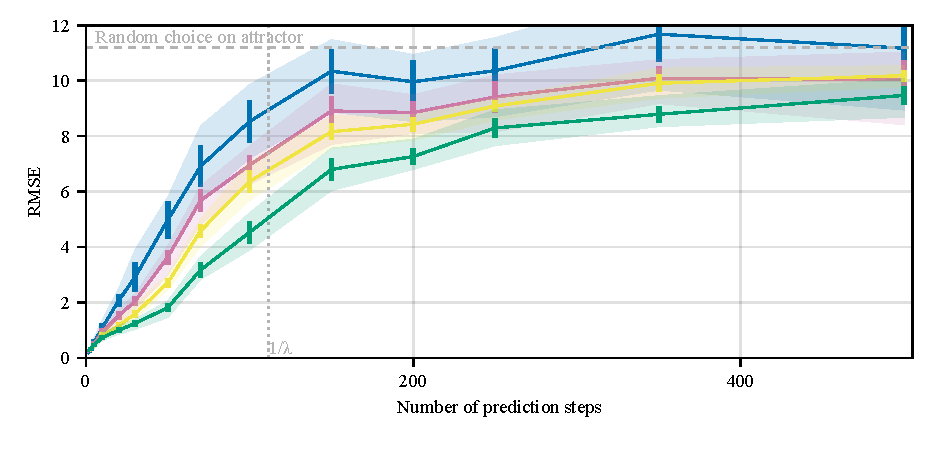
\includegraphics[width=1.1\textwidth,trim=0 8mm 0 0,clip]{../Images/ORSESN/ORSESN_topline_recursive_Lorenz 0_01.pdf}
        }
    \end{subfigure}

    \vspace{0.5em}

    \begin{subfigure}{\textwidth}
        \caption{Mean iterative prediction RMSE on the Lorenz series with time step size $\Delta t=0.05$ for the ORSESN with delays $\tau=10,10,4$ for $m=2,3,4$ respectively, noise level $\alpha=0.1$, and total reservoir size $k=500$.}
        \label{fig:ORSESN_iterative_0_05}
        \centering
        \makebox[\textwidth][c]{%
            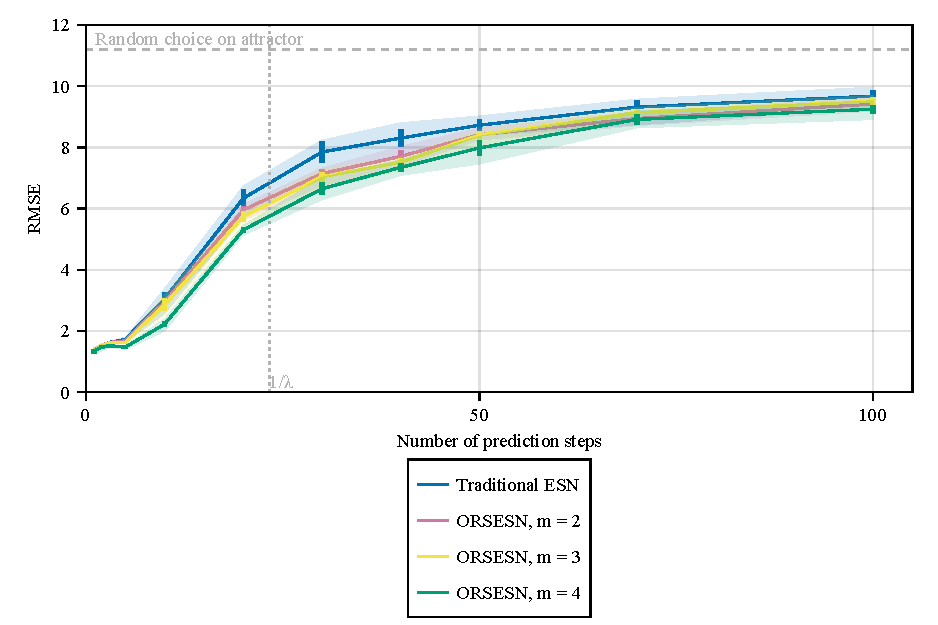
\includegraphics[width=1.1\textwidth]{../Images/ORSESN/ORSESN_topline_recursive_Lorenz 0_05.pdf}
        }
    \end{subfigure}

    % \caption{Mean iterative prediction RMSE for the ORSESN for Lorenz x component time series with two different time steps: (a) $\Delta t=0.01$ and (b) $\Delta t=0.05$, both with additive noise $\alpha=0.1$, delay $\tau=20$ and total reservoir size $k=468$. The standard deviations between trials are represented by vertical bars and the range of trial results is represented by the shaded regions.}
    \caption{Mean iterative prediction RMSE for the ORSESN on the Lorenz $x$-component time series with additive noise $\alpha=0.1$ and total reservoir size $k=500$. Subfigure (a) shows results for time step size $\Delta t=0.01$, delay $\tau=20$ for all $m$; subfigure (b) shows results for time step size $\Delta t=0.05$, delays $\tau=10,10,4$ for $m=2,3,4$, respectively. Standard deviations between trials are represented by vertical bars and shaded regions indicate the full range of trial results.}
\end{figure}



\subsection{Lorenz - direct prediction}


Here we will analyse the ability of the ORSESN to generate direct predictions. For the Lorenz system with time step size $\Delta t=0.01$, as shown in Figure \ref{fig:ORSESN_direct_0_01}, the traditional ESN initially performs well for short prediction horizons, achieving a mean RMSE of 0.228 ($\pm 0.033$) after 1 step. The ORSESN models show slightly higher errors at this prediction length, with mean RMSEs of 0.243 ($\pm 0.020$), 0.233 ($\pm 0.017$), and 0.228 ($\pm 0.021$) for $m=2$, $m=3$, and $m=4$, respectively. But mirroring what we observed in the iterative predictions, the ORSESN models perform better at longer prediction lengths. At 20 prediction steps, all three ORSESN models achieve a statistically significant (95\% CI) lower mean RMSE than the traditional ESN, with a higher $m$ producing a lower RMSE over the whole tested range of prediction lengths.

For direct prediction on the Lorenz system with time step size $\Delta t=0.05$ (Figure \ref{fig:ORSESN_direct_0_05}), the ORSESN with $m=4$ outperforms the traditional ESN from the start (mean RMSE of $0.239\pm 0.019$ vs. $0.311\pm 0.025$ at 1 step) and maintains this advantage throughout longer horizons ($0.759\pm 0.045$ vs. $1.175\pm 0.076$ at 5 steps; $5.003\pm 0.088$ vs. $6.214\pm 0.254$ at 20 steps). The ORSESN with $m=3$ also reliably outperforms the traditional ESN, however the ORSESN with $m=2$ fails to significantly improve (95\% CI) the traditional ESN at many prediction lengths.

Both direct and iterative prediction methods confirm the same conclusion: while traditional ESNs are superior or on-par for short-term forecasts, the ORSESN provides more accurate and stable predictions for medium to long-term horizons, with performance improving as the ordinal pattern dimension increases. The direct prediction results further confirm that the ORSESN's superior performance is not an artifact of error accumulation in iterative prediction but rather reflects a genuine improvement in the model's ability to capture the underlying dynamics of the chaotic system. There is a consistent pattern of lower errors for the ORSESN at longer prediction horizons across both forms of prediction.


\begin{figure}
    \centering

    \begin{subfigure}{\textwidth}
        \caption{Mean direct prediction RMSE on the Lorenz series with time step size $\Delta t=0.01$ for the ORSESN with delay $\tau=20$, noise level $\alpha=0.1$, and total reservoir size $k=500$.}
        \label{fig:ORSESN_direct_0_01}
        \centering
        \makebox[\textwidth][c]{%
            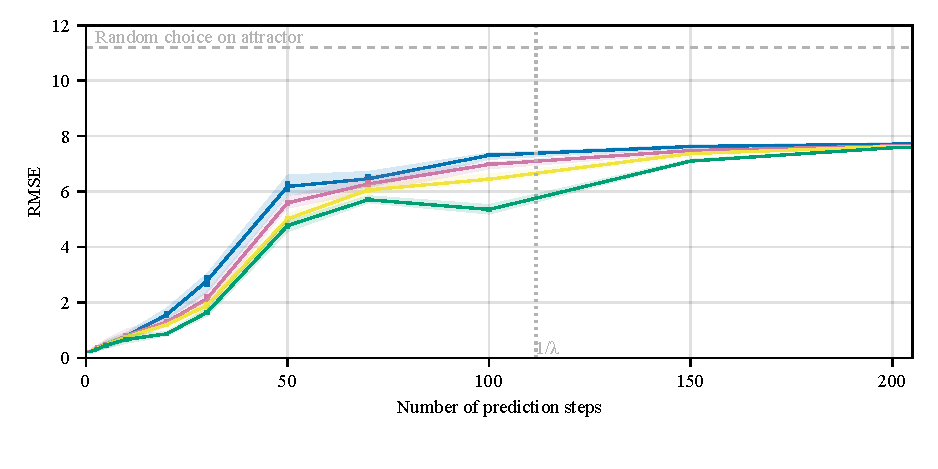
\includegraphics[width=1.1\textwidth,trim=0 8mm 0 0,clip]{../Images/ORSESN/ORSESN_topline_direct_Lorenz 0_01.pdf}
        }
    \end{subfigure}

    \vspace{0.5em}

    \begin{subfigure}{\textwidth}
        \caption{Mean direct prediction RMSE on the Lorenz series with time step size $\Delta t=0.05$ for the ORSESN with delay $\tau=4$, noise level $\alpha=0.1$, and total reservoir size $k=500$.}
        \label{fig:ORSESN_direct_0_05}
        \centering
        \makebox[\textwidth][c]{%
            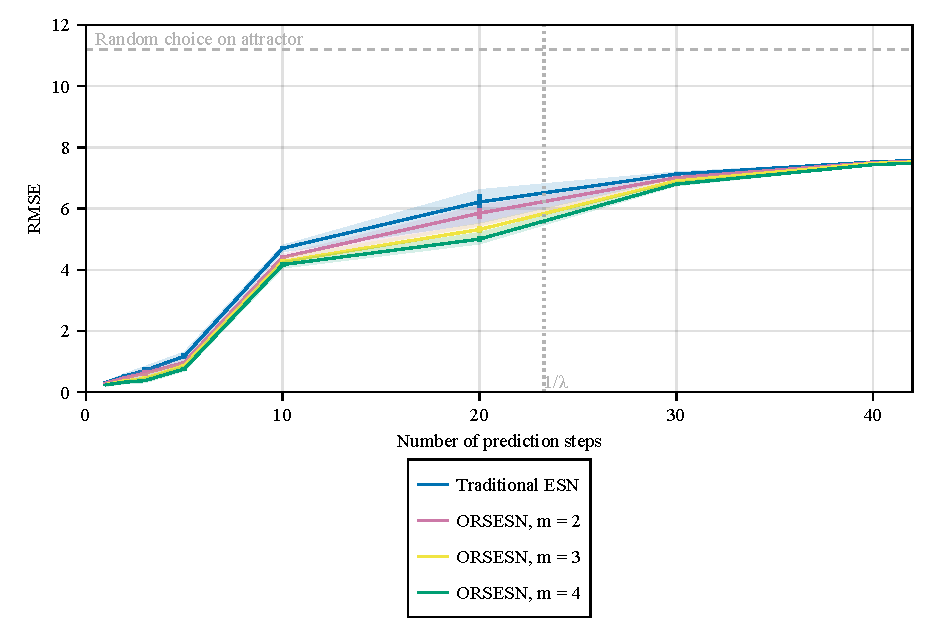
\includegraphics[width=1.1\textwidth]{../Images/ORSESN/ORSESN_topline_direct_Lorenz 0_05.pdf}
        }
    \end{subfigure}

    \caption{Mean direct prediction RMSE for the ORSESN on the Lorenz $x$-component time series with additive noise $\alpha=0.1$ and total reservoir size $k=500$. Subfigure (a) shows results for time step size $\Delta t=0.01$, delay $\tau=20$ for all $m$; subfigure (b) shows results for time step size $\Delta t=0.05$, delay $\tau=4$ for all $m$. Standard deviations between trials are represented by vertical bars and shaded regions indicate the full range of trial results.}
    \label{fig:ORSESN_direct}
\end{figure}



\subsection{Comparison across attractors}

\subsubsection{R\"ossler system}

For the R\"ossler system integrated with a time step size of $\Delta t=0.1$ (Figure~\ref{fig:ORSESN_rossler_iterative}), the results show a similar pattern to the Lorenz attractor. The traditional ESN exhibits lower error for very short term predictions, but after 5 recursive steps the mean RMSE of the ORSESN with $m=4$ ($0.374 \pm 0.0190$) and $m=3$ ($0.385 \pm 0.022$) significantly (95\% CI) outperform the traditional ESN ($0.482 \pm 0.041$). Like those predictions for the Lorenz series, this advantage becomes more pronounced at longer horizons; for instance, at 200 steps, ORSESN with $m=4$ achieves a significantly lower mean RMSE of 2.176 ($\pm 0.250$) compared to 4.393 ($\pm 1.126$) for the traditional ESN. Furthermore, the ORSESN with $m=4$ demonstrates remarkable prediction stability at this horizon, with a standard deviation of only 0.250, whereas the traditional ESN has a standard deviation of 1.126.

The ORSESN with $m=2$ fails to be significantly more accurate at multiple prediction lengths, and the ORSESN with $m=3$ provides insignificant improvement after 150 prediction steps. After 200 prediction steps, the ORSESN with $m=4$ no longer significantly outperforms the traditional ESN, but this can be seen to be a result of the higher standard deviation in the results of the traditional ESN.

Comparing these findings with the Lorenz system, the general performance characteristics are consistent. Traditional ESNs tend to be more accurate for shorter prediction lengths, however ORSESN models outperform on accuracy and stability for longer predictions lengths, particularly where $m=4$.
The crossover point, where ORSESN models begin to outperform traditional ESNs, typically occurs within the first 10 prediction steps for both chaotic systems.

What appears peculiar is the comparably low mean RMSE and small variance of the ORSESN with $m=4$. Figure \ref{fig:ORSESN_rossler_freerun} shows iterative predictions over 200 prediction steps (Rossler with $\Delta t = 0.1$) for the ORSESN and traditional ESN. Simply inspecting these predictions, all four models appear to predict the dynamics of only approximately one cycle before reverting to an `average' periodic prediction. However the ORSESN with $m=4$ appears to be able to predict the dynamics of 2 to 3 cycles to varying degrees of success before reverting to the `average' periodic prediction.



\begin{figure}
    \centering

    \centering
    \makebox[\textwidth][c]{%
        \includegraphics[width=1.1\textwidth,trim=0 0 0 0,clip]{../Images/ORSESN/ORSESN_topline_recursive_rossler 0_1.pdf}
    }

    \caption{Mean iterative prediction RMSE for the ORSESN for R\"ossler $x$ component time series with time step size $\Delta t=0.1$ and additive noise $\alpha=0.1$, delay $\tau=20$ and total reservoir size $k=500$. The standard deviations between trials are represented by vertical bars and the range of trial results is represented by the shaded regions.}
    \label{fig:ORSESN_rossler_iterative}
\end{figure}

\begin{figure}
    \centering
    \makebox[\textwidth][c]{%
        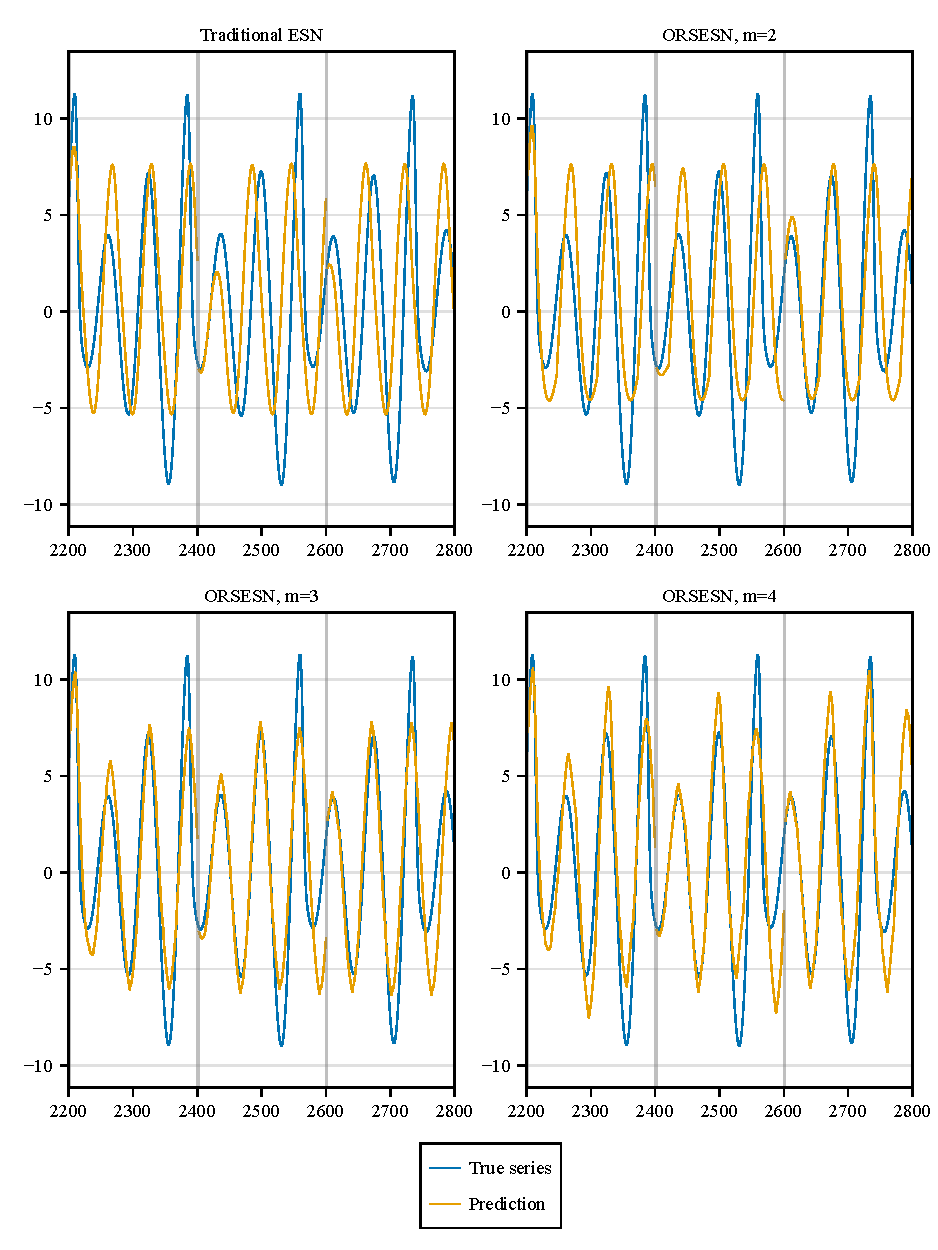
\includegraphics[width=1\textwidth,trim=0 0 0 0,clip]{../Images/ORSESN/ORSESN_freerun_recursive_Rossler.pdf}
    }
    \caption{Iterative free-run predictions for the Rössler system ($x$ component) with time step size $\Delta t=0.1$. The figure compares the traditional ESN with ORSESN models of varying ordinal pattern dimensions ($m=2,3,4$) over 200 prediction steps. All models were configured with a delay $\tau=20$, additive noise $\alpha=0.1$, and a total reservoir size $k=500$. Each grey vertical line indicates the beginning of prediction chunk, where the echo state network changes from being driven by the true signal to being driven by its own predictions.}
    \label{fig:ORSESN_rossler_freerun}
\end{figure}



The direct prediction performance on the Rössler system (Figure \ref{fig:ORSESN_rossler_direct}) is consistent with the iterative prediction trends. The benefit of the ORSESN appears more pronounced for the Rossler time series than the Lorenz time series.
Direct predictions on the Rossler series again shows the traditional ESN with slightly lower error for short predictions but the ORSESN models with higher ordinal pattern dimensions ($m$) generally achieve better accuracy for longer predictions. At 20 prediction steps, ORSESN with $m=4$ (mean RMSE $0.701\pm 0.058$) is significantly (95\%CI) more accurate than the traditional ESN (mean RMSE $1.094\pm 0.155$).
The mean prediction RMSE for all models converges, similar to the direct predictions for the Lorenz series, at approximately 350 prediction steps.
% A prediction at this length simply reflects the ESN's ability to match the periodicity of the data rather than its ability to represent the dynamics of the attractor.


\begin{figure}

    \centering
    \makebox[\textwidth][c]{%
        \includegraphics[width=1.1\textwidth,trim=0 0 0 0,clip]{../Images/ORSESN/ORSESN_topline_direct_rossler 0_1.pdf}
    }

    \caption{Mean direct prediction RMSE for the ORSESN for R\"ossler $x$ component time series with time step size $\Delta t=0.1$ and additive noise $\alpha=0.1$, delay $\tau=20$ and total reservoir size $k=500$. The standard deviations between trials are represented by vertical bars and the range of trial results is represented by the shaded regions.}
    \label{fig:ORSESN_rossler_direct}
\end{figure}



\subsubsection{Mackey-Glass system}

% apple
The iterative prediction results for the Mackey-Glass system with a time step size $\Delta t=0.5$ are illustrated in Figure \ref{fig:ORSESN_mg_iterative}.
Like the Lorenz and R\"ossler attractors, the traditional ESN demonstrates a clear advantage in single time step prediction for this system.

Similarly again, the ORSESN models generally show significantly (95\% CI) improved performance over the traditional ESN as the prediction horizon grows. For instance, at 20 recursive prediction steps, the traditional ESN has a mean RMSE of 0.110 ($\pm 0.010$), while the ORSESN with $m=2$ achieves 0.071 ($\pm 0.003$), $m=3$: 0.070 ($\pm 0.003$), and $m=4$: 0.039 ($\pm 0.001$).

Unlike the other attractors, the ORSESN models with $m=2$ and $m=3$ maintain significantly (95\% CI) improved accuracy only up to around 70 prediction steps, while the ORSESN with $m=4$ continues to provide improved accuracy for much longer predictions.

The ORSESN with $m=4$ achieves a consistent significantly (95\% CI) improved accuracy for all tested prediction lengths 5 time steps or longer. It maintains a much lower mean RMSE and a smaller standard deviation compared to both the traditional ESN and the other ORSESN configurations ($m=2,3$) for longer prediction horizons. For example, the performance at 100 steps is 62\% lower in error than the traditional ESN at 100 steps, with standard deviation of 0.002 much lower than the traditional ESN's 0.017. An example of the prediction of all four models can be found in Figure \ref{fig:ORSESN_mg_freerun}, however unlike the Rossler system, a simple qualitative explanation for the outperforming ORSESN with $m=4$ is not apparent.

\begin{figure}
    \centering

    % \begin{subfigure}{\textwidth}
        % \caption{Mean iterative prediction RMSE on the Mackey-Glass series with time step $\Delta t=0.5$ for the ORSESN with delay $\tau=20$.}
        % \label{fig:ORSESN_mg_iterative_0_5}
        % \centering
        \makebox[\textwidth][c]{%
            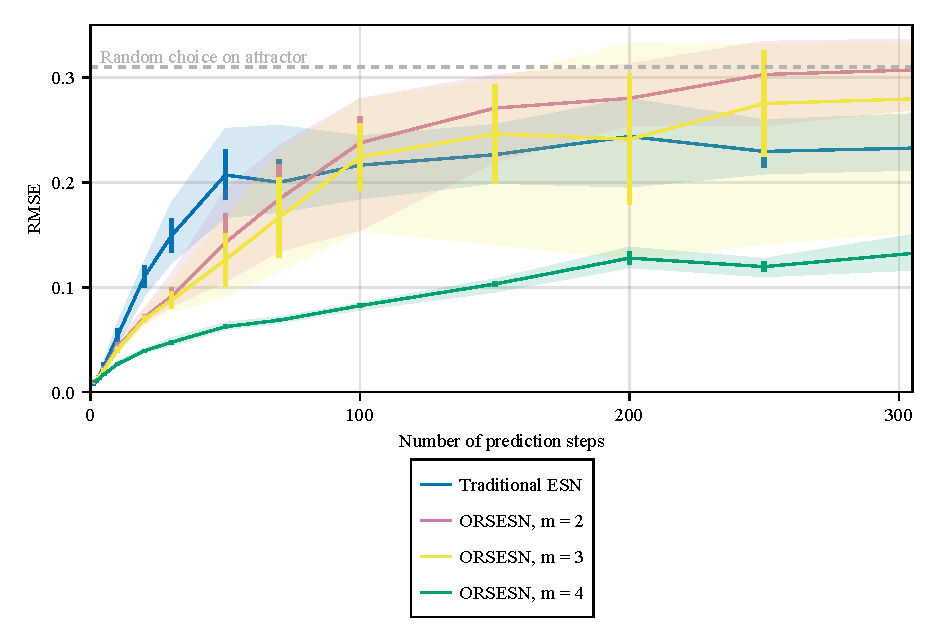
\includegraphics[width=1.1\textwidth,trim=0 0 0 0,clip]{../Images/ORSESN/ORSESN_topline_recursive_MG 0_5.pdf}
        }
    % \end{subfigure}

    % \vspace{0.5em}

    % \begin{subfigure}{\textwidth}
    %     \caption{TODO MORE TRIALS AND LONGER TEST SERIES Mean iterative prediction RMSE on the Mackey-Glass series with time step $\Delta t=2.5$ for the ORSESN with delay $\tau=50$.}
    %     \label{fig:ORSESN_mg_iterative_2_5}
    %     \centering
    %     \makebox[\textwidth][c]{%
    %         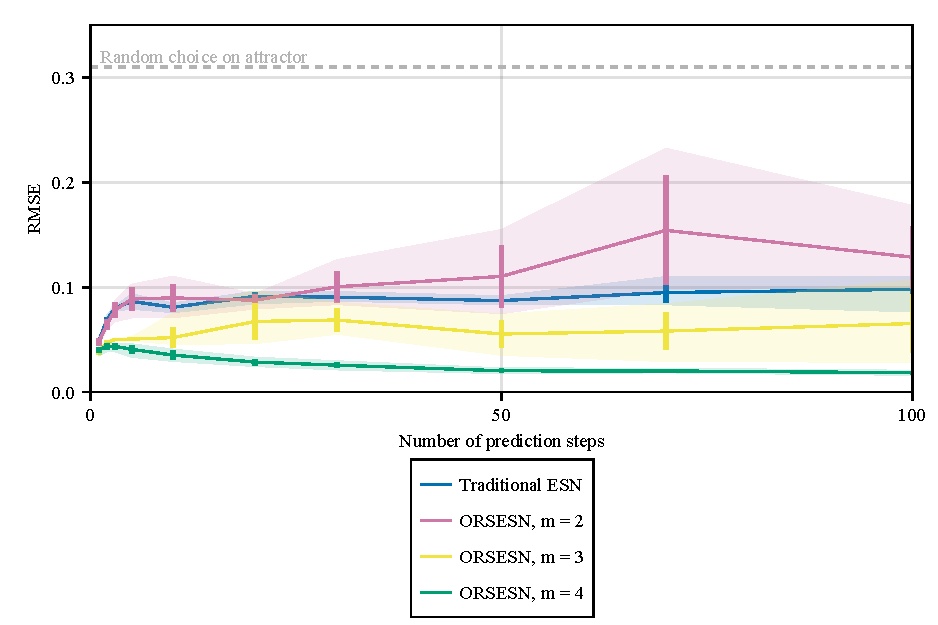
\includegraphics[width=1.1\textwidth]{../Images/ORSESN/ORSESN_topline_recursive_MG 2_5.pdf}
    %     }
    % \end{subfigure}

    % \caption{Iterative prediction RMSE for the ORSESN for Mackey-Glass time series with two different time steps: (a) $\Delta t=0.5$ (delay $\tau=20$) and (b) $\Delta t=2.5$ (delay $\tau=50$), both with additive noise $\alpha=0.1$ and total reservoir size $k=468$. The standard deviations between trials are represented by vertical bars and the range of trial results is represented by the shaded regions.}
    \caption{Iterative prediction RMSE for the ORSESN for Mackey-Glass time series with $\Delta t=0.5$, delay $\tau=20$, additive noise $\alpha=0.1$ and total reservoir size $k=500$. The standard deviations between trials are represented by vertical bars and the range of trial results is represented by the shaded regions.}
    \label{fig:ORSESN_mg_iterative}
\end{figure}

\begin{figure}
    \centering
    \makebox[\textwidth][c]{%
        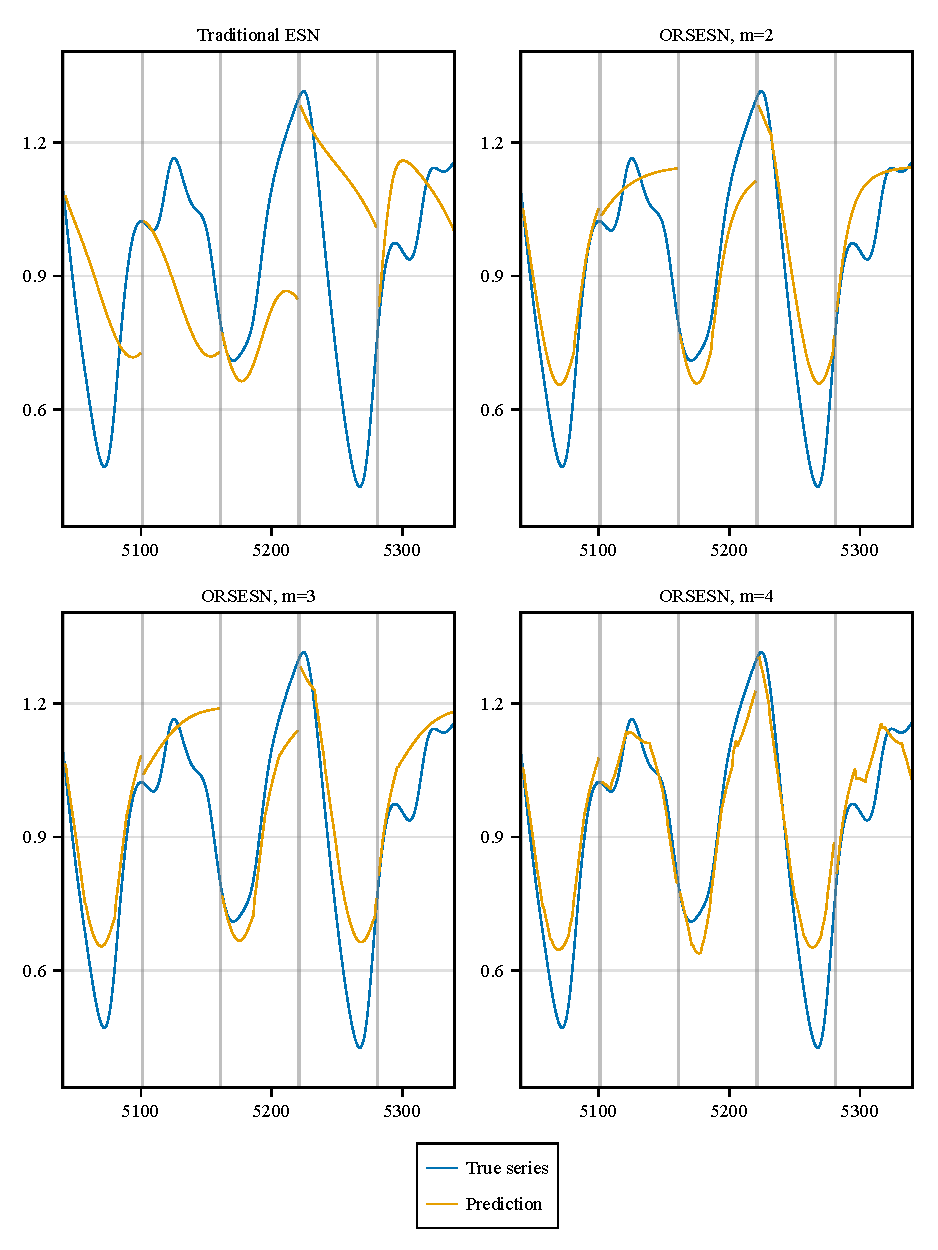
\includegraphics[width=1\textwidth]{../Images/ORSESN/ORSESN_freerun_recursive_Mackey_Glass.pdf}%
    }
    \caption{Example of iterative prediction for the Mackey-Glass system ($\Delta t=0.5$, additive noise $\alpha=0.1$). Predictions from the traditional ESN ($m=1, \tau=1$) and ORSESN ($m \in \{2,3,4\}, \tau=20$) are compared against the true series. All models use a total reservoir size $k=500$. Each grey vertical line indicates the beginning of prediction chunk, where the echo state network changes from being driven by the true signal to being driven by its own predictions.}
    \label{fig:ORSESN_mg_freerun}
\end{figure}

% apple
The direct prediction results for the Mackey-Glass system (Figure \ref{fig:ORSESN_mg_direct}) show a clear and consistent trend: the ORSESN produces a consistently lower mean RMSE, with $m=4$ achieving a significantly (95\%CI) superior result across all tested prediction lengths. This contrasts with the iterative prediction setting, where the advantage of higher $m$ is limited to shorter horizons and can degrade at longer ones; direct prediction has no crossover or degradation of performance for $m=2$ or $m=3$ at longer steps.

These results suggest that while the ORSESN with $m=2$ and $m=3$ can initially outperform the traditional ESN for medium length iterative predictions, they may be less effective at correcting for accumulating errors as the prediction length grows. This behavior leads to a crossover where the traditional ESN eventually matches or surpasses their performance.

However, this limitation is mitigated when the ordinal pattern dimension is increased to $m=4$. The ORSESN with $m=4$ not only maintains its initial advantage but also demonstrates sustained accuracy and stability across all tested prediction horizons. The mean RMSE for the $m=4$ ORSESN is 66\% lower than the traditional ESN at 10 direct prediction steps, and 51\% lower at 100 direct prediction steps. This indicates that a higher ordinal pattern dimension enables the ORSESN to capture more relevant dynamical information, resulting in both improved short term accuracy and greater resilience to error accumulation in long term predictions.




\begin{figure}
    \centering

    % \begin{subfigure}{\textwidth}
    %     \caption{Mean direct prediction RMSE on the Mackey-Glass series with time step $\Delta t=0.5$ for the ORSESN with delay $\tau=20$.}
    %     \label{fig:ORSESN_mg_direct_0_5}
    %     \centering
        \makebox[\textwidth][c]{%
            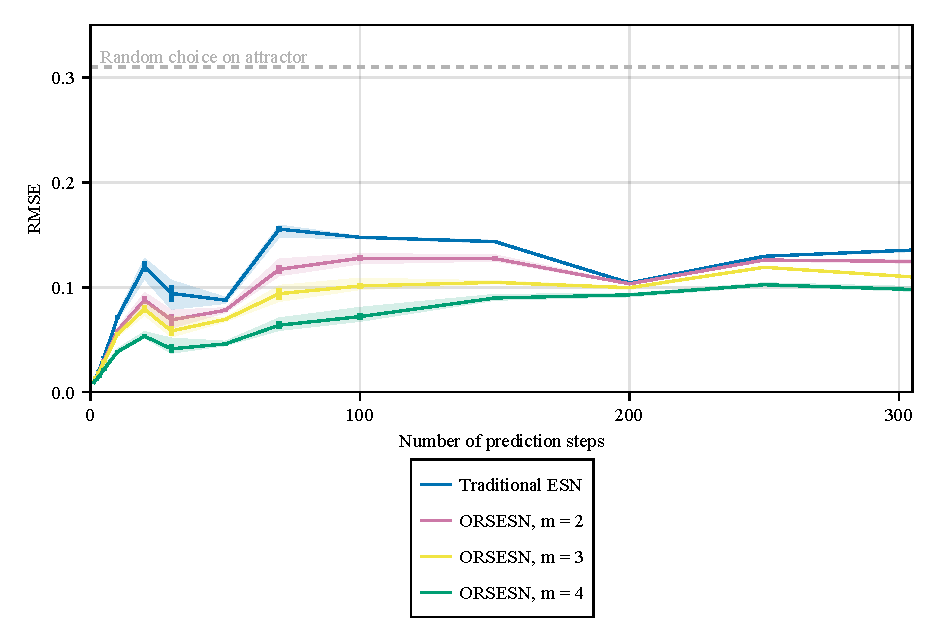
\includegraphics[width=1.1\textwidth]{../Images/ORSESN/ORSESN_topline_direct_MG 0_5.pdf}
        }
    % \end{subfigure}

    % \vspace{0.5em}

    % \begin{subfigure}{\textwidth}
    %     \caption{TODO MORE TRIALS AND LONGER TEST SERIES Mean direct prediction RMSE on the Mackey-Glass series with time step $\Delta t=2.5$ for the ORSESN with delays $\tau=50,50,20$ for $m=2,3,4$ respectively.}
    %     \label{fig:ORSESN_mg_direct_2_5}
    %     \centering
    %     \makebox[\textwidth][c]{%
    %         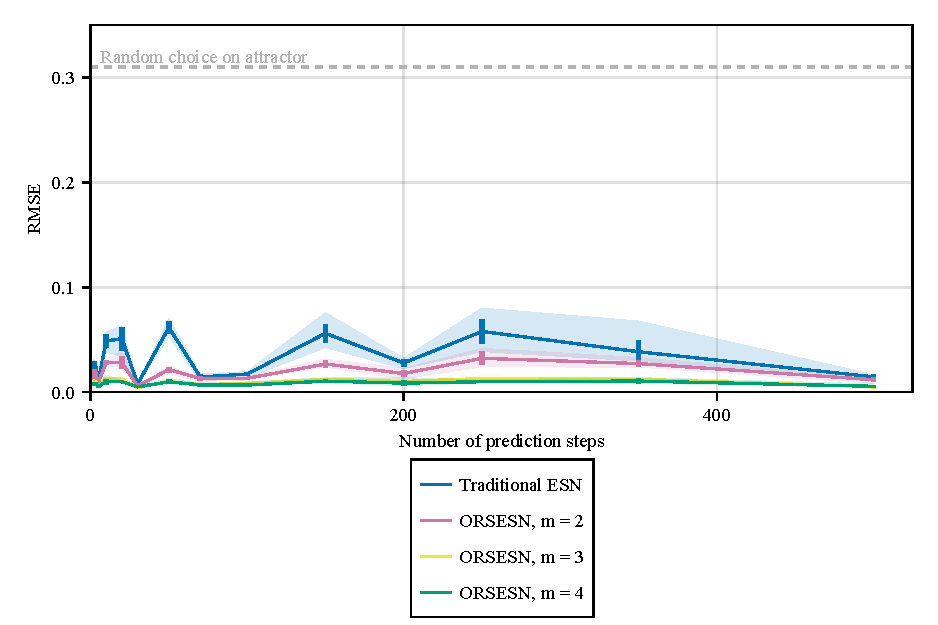
\includegraphics[width=1.1\textwidth]{../Images/ORSESN/ORSESN_topline_direct_MG 2_5.pdf}
    %     }
    % \end{subfigure}

    % \caption{Mean direct prediction RMSE for the ORSESN for Mackey-Glass time series with two different time steps: (a) $\Delta t=0.5$ (delay $\tau=20$) and (b) $\Delta t=2.5$ (delay $\tau=50$), both with additive noise $\alpha=0.1$ and total reservoir size $k=468$. The standard deviations between trials are represented by vertical bars and the range of trial results is represented by the shaded regions.}
    \caption{Mean direct prediction RMSE for the ORSESN for Mackey-Glass time series with $\Delta t=0.5$, delay $\tau=20$, additive noise $\alpha=0.1$ and total reservoir size $k=500$. The standard deviations between trials are represented by vertical bars and the range of trial results is represented by the shaded regions.}
    \label{fig:ORSESN_mg_direct}
\end{figure}





\subsection{Gating}


The ORSESN introduces a new architectural feature, the readout gating mechanism, and drives the gating using ordinal partition information of the incoming data. We would like to confirm whether it is the ordinal partition information that is creating the improved predictions rather than just the gating mechanism itself. To test this, we supplied the ORSESN with the Lorenz time series with $\Delta t=0.01$ accompanied by a random selection of the readout and compared it to the readout selection driven by the ordinal partition. Figure \ref{fig:ORSESN_routing_ordinal_vs_random} shows the performance of the ORSESN when its readout is gated via the ordinal partitions of the data compared to its performance when the gating of the readout is determined by random selection, for each of $m=2,3,4$. The performance of the ORSESN with random gating is insignificantly (95\% CI) different from the performance of our traditional ESN benchmark, with the mean RMSE value across trials lying within one standard deviation of the traditional ESN across all tested lengths of iterative prediction. We can infer from this testing that the predictive advantage of the ORSESN is likely conferred by the ordinal partition information rather than the use of the multiple readout vector gating mechanism by itself.

\begin{figure}
    \centering

    \begin{subfigure}{\textwidth}
        \caption{ORSESN Readout Gating - Ordinal Partition Driven vs. Random Selection, $m=2$}
        \label{fig:ORSESN_routing_m_2}
        \centering
        \makebox[\textwidth][c]{%
            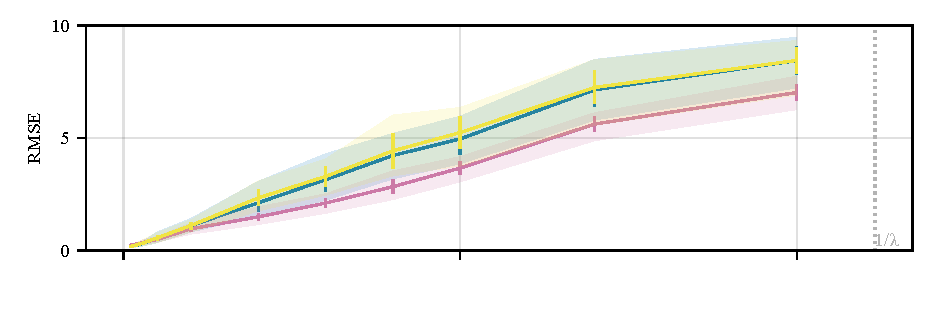
\includegraphics[width=1.1\textwidth,trim=0 0 0 3mm,clip]{../Images/ORSESN/ORSESN_routing_ordinal_vs_random_m=2.pdf}%
        }
    \end{subfigure}

    \vspace{0em}

    \begin{subfigure}{\textwidth}
        \caption{ORSESN Readout Gating - Ordinal Partition Driven vs. Random Selection, $m=3$}
        \label{fig:ORSESN_routing_m_3}
        \centering
        \makebox[\textwidth][c]{%
            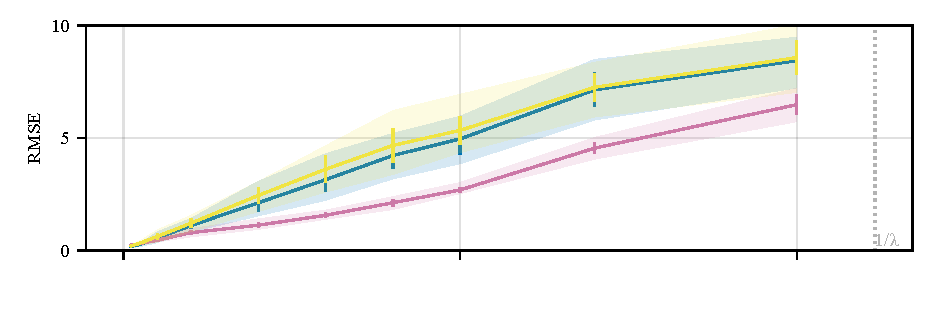
\includegraphics[width=1.1\textwidth,trim=0 0 0 3mm,clip]{../Images/ORSESN/ORSESN_routing_ordinal_vs_random_m=3.pdf}%
        }
    \end{subfigure}

    \vspace{0em}

    \begin{subfigure}[t]{\textwidth}
        \caption{ORSESN Readout Gating - Ordinal Partition Driven vs. Random Selection, $m=4$}
        \label{fig:ORSESN_routing_m_4}
        \centering
        \makebox[\textwidth][c]{%
            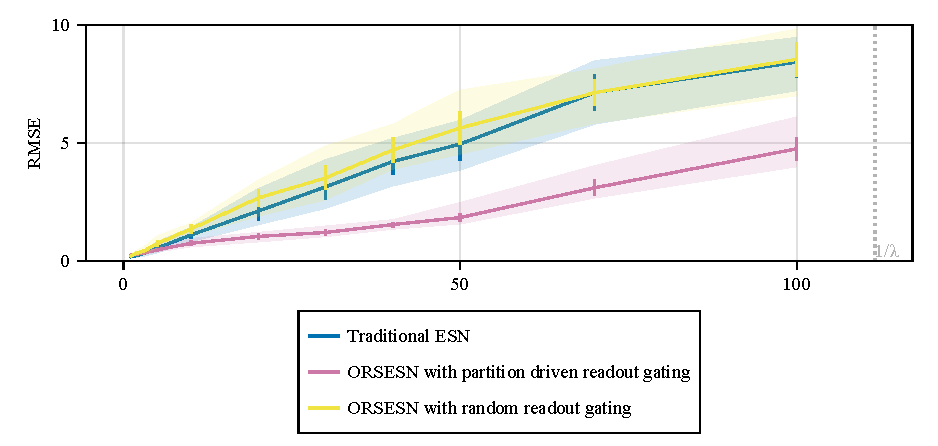
\includegraphics[width=1.1\textwidth,trim=0 0 0 3mm,clip]{../Images/ORSESN/ORSESN_routing_ordinal_vs_random_m=4.pdf}%
        }
    \end{subfigure}

    % \caption{Mean iterative prediction RMSE across trials for the ORSESN compared with a variant that chooses the readout randomly rather than dependent on the ordinal partition of the input, for delay $\tau=20$, noise level $\alpha=0.1$, and total reservoir size $k=468$. Subfigures (a), (b), and (c) correspond to $m=2$, $m=3$, and $m=4$, respectively. The standard deviations between trials are represented by vertical bars and the range of trial results is represented by the shaded regions.}
    \caption{Mean iterative prediction RMSE across trials for the ORSESN on the Lorenz $x$-component time series with time step size $\Delta t=0.01$, delay $\tau=20$, additive noise $\alpha=0.1$, and total reservoir size $k=468$, compared to a variant that selects the readout randomly rather than by ordinal partition. Subfigures (a), (b), and (c) correspond to $m=2$, $m=3$, and $m=4$, respectively. Standard deviations between trials are represented by vertical bars and shaded regions indicate the full range of trial results.}
    \label{fig:ORSESN_routing_ordinal_vs_random}
\end{figure}



\subsection{Resilience to noise}

We can test the resilience of models to noise by adding increasing levels of noise to the training data and testing the resulting prediction performance. We can then compare the effect of noise on the model's ability to create predictions. Figure \ref{fig:ORSESN_noise_resilience_direct} shows the mean direct prediction RMSE of multiple trials across values of noise $\alpha\in[0.0, 1.0]$, with four curves representing different numbers of prediction steps. As to be expected, as the level of noise increases so does the prediction RMSE for both the traditional ESN ($m=1$) and the ORSESN models ($m=2,3,4$). Compared to the traditional ESN, the ORSESN models appear to be less resilient to noise as the relative increase in RMSE is greater over noise levels $0.0$ to $1.0$. However the absolute mean RMSE is still lower (or approximately equal) for all $\alpha \in [0.0, 1.0]$ despite this lesser resilience to noise.

\begin{figure}
    \centering
    % ensure the graphic is centered and scaled to the text width without overflow
    \makebox[\textwidth][c]{%
        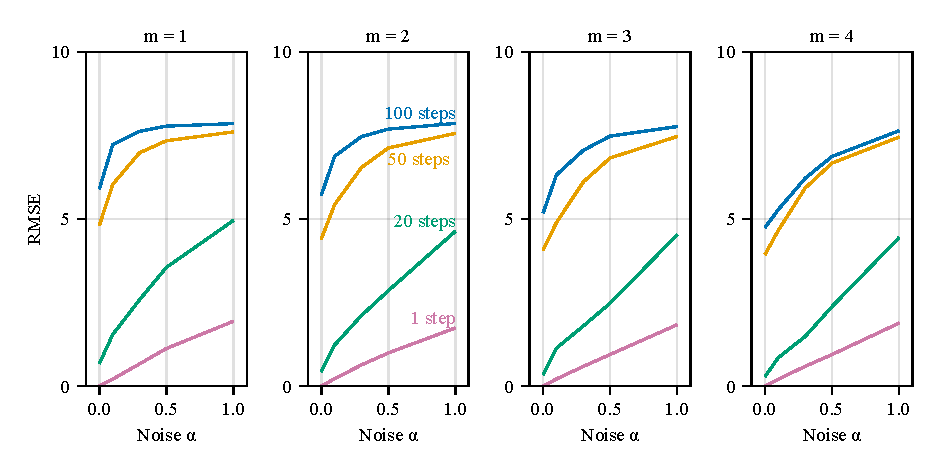
\includegraphics[width=1.1\textwidth]{../Images/ORSESN/ORSESN_direct_noise_resilience.pdf}%[width=1.2\textwidth]
    }%[width=\textwidth,keepaspectratio]
    % \caption{Mean direct prediction RMSE across trials for the OPESN as a function of simulated data noise level $\alpha$, with delay $\tau=20$ and reservoir size $k=468$. Curves correspond to different numbers of prediction steps, and each axis represents an ORSESN with a different value for $m$. The axis labeled $m=1$ refers to the traditional ESN.}
    \caption{Mean direct prediction RMSE across trials for the ORSESN on the Lorenz $x$-component time series with time step size $\Delta t=0.01$ as a function of simulated data noise level $\alpha$, with delay $\tau=20$ and total reservoir size $k=468$. Curves correspond to different numbers of prediction steps, and each panel represents an ordinal pattern dimension $m$ (with $m=1$ denoting the traditional ESN).}
    \label{fig:ORSESN_noise_resilience_direct}
\end{figure}

Figure \ref{fig:ORSESN_noise_resilience_iterative} shows the same noise analysis performed with iterative prediction instead of direct prediction. Iterative prediction yields similar results, where the traditional ESN appears to be more resilient to noise however the ORSESN has a lower (or approximately the same) mean prediction RMSE for $0.0 \leq \alpha \leq 1.0$. The reader can see that as the noise level increases, the predictive performance initially improves between $\alpha = 0.0$ and $\alpha = 0.1$ before degrading between $\alpha = 0.1$ and $\alpha = 1.0$. This `sweet spot' has been observed previously, where a modest amount of noise in training data lowers the prediction error of an ESN when producing iterative predictions~\cite{jaeger_2001}\cite{lukosevicius_and_jaeger_2009}. The benefit has been interpreted as a `mild stochastic regularisation', broadening the set of states seen during training so that the readout is less likely to compound small errors during iterative prediction. For the purposes of testing the performance of the traditional ESN and the ORSESN we have chosen the `sweet spot' value of $\alpha = 0.1$.

\begin{figure}
    \centering
    % ensure the graphic is centered and scaled to the text width without overflow
    \makebox[\textwidth][c]{%
        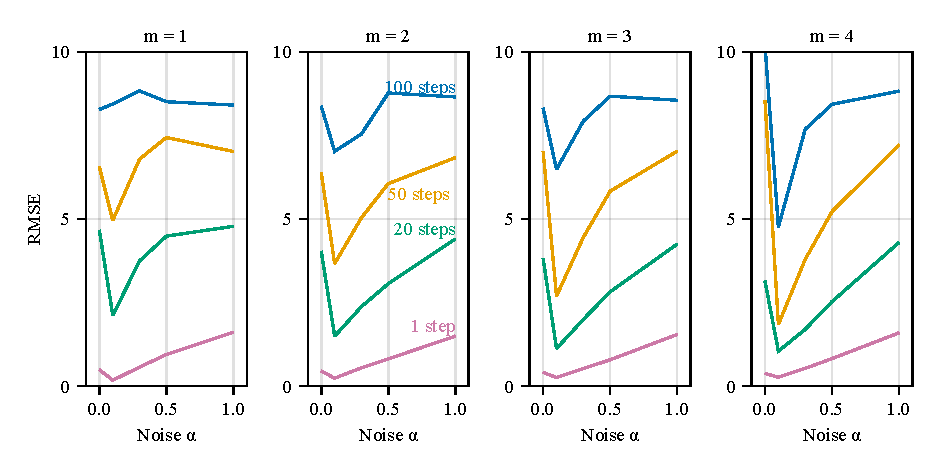
\includegraphics[width=1.1\textwidth]{../Images/ORSESN/ORSESN_recursive_noise_resilience.pdf}%[width=1.2\textwidth]
    }%[width=\textwidth,keepaspectratio]
    % \caption{Iterative prediction RMSE for the ORSESN as a function of simulated data noise level $\alpha$, with delay $\tau=20$ and reservoir size $k=468$. Curves correspond to different numbers of prediction steps, and each axis represents an ORSESN with a different value for $m$. The axis labeled $m=1$ refers to the traditional ESN.}
    \caption{Mean iterative prediction RMSE across trials for the ORSESN on the Lorenz $x$-component time series with time step size $\Delta t=0.01$ as a function of simulated data noise level $\alpha$, with delay $\tau=20$ and total reservoir size $k=468$. Curves correspond to different numbers of prediction steps, and each panel represents an ordinal pattern dimension $m$ (with $m=1$ denoting the traditional ESN).}
    \label{fig:ORSESN_noise_resilience_iterative}
\end{figure}

In an effort to explain this result, one should note that ordinal partitions are invariant to monotonic transformations but they are not immune to misclassification when the signal is noisy. Figures \ref{fig:ORSESN_noise_resilience_direct} and \ref{fig:ORSESN_noise_resilience_iterative} show that prediction error grows faster with $\alpha$ for ORSESN than for the traditional ESN, because additive noise can flip the relative order of nearby samples and therefore trigger an incorrect readout. In other words, as we increase $\alpha$ we are pushing the gating mechanism to become random - the effects of which have been tested above. Nevertheless ORSESN preserves an absolute advantage up to $\alpha=1.0$ in the present setting, implying that its gains outweigh the extra sensitivity unless measurement noise is extreme. For applications where noise cannot be pre-filtered, a softened gating strategy such as weighting readouts by the posterior probability of each partition rather than enforcing a hard mask may retain accuracy while dampening the noise penalty.



\subsection{Extended discussion}

Across all three benchmark systems, the traditional ESN delivers the lowest error at the one-step horizon, but the ORSESN with ordinal dimension $m = 4$ steadily outperforms it for medium and long-term forecasts. We suggest this arises from the different ways each model embeds past inputs: the ESN's echo state property produces a fading-memory embedding that weights recent samples more than past samples, while a backward ordinal pattern of length $m\tau + 1$ encodes all samples in its window equally. In the ORSESN, separate readouts are trained on states gated by each ordinal partition - reducing the data per readout but ensuring that each specializes on homogeneous dynamical conditions. For short predictions, the ESN's single readout trained on the full set of reservoir states interprets the dynamics of the recency biased reservoir more effectively. By contrast, the ORSESN's partitioned readouts each receive less training data and may underfit, resulting in poorer short-term accuracy. For extended horizons, however, the ORSESN readouts capture longer-timescale structure, counteract the ESN's biased memory, and thus yield more accurate medium and long-term predictions.

The random-gating experiment (Figure \ref{fig:ORSESN_routing_ordinal_vs_random}) confirms that the improvement stems from the ordinal structure, not from the mere presence of multiple readouts. Thus the ORSESN not only provides strong evidence that ordinal partitions are an effective predictive feature for ESNs, but is also an effective architecture to take advantage of this feature.
